%%%%%%%%%%%%%%%%%%%%%%%%%%%%%%%%%%%%%%%%%%%%%%%%%%%%%%%%%%%%%%%%%%%%
%% Presentation: Diabetic Retinopathy Detection and Classification
%%%%%%%%%%%%%%%%%%%%%%%%%%%%%%%%%%%%%%%%%%%%%%%%%%%%%%%%%%%%%%%%%%%%

\documentclass{beamer}
\usetheme[faculty=wi]{fibeamer}
\usepackage[utf8]{inputenc}
\usepackage[
  main=vietnamese,
  vietnamese
]{babel}

\title{Xác định mức độ và phân đoạn thương tổn của bệnh võng mạc tiểu đường bằng mạng CNN}
\date{\today}

\usepackage{ragged2e}
\usepackage{booktabs}
\usepackage{tabularx}
\usepackage{tikz}
\usetikzlibrary{calc, shapes, backgrounds, positioning}
\usepackage{amsmath, amssymb}
\usepackage{url}
\usepackage{graphicx}
% Search graphics in outputs folders relative to this .tex file
\graphicspath{{../outputs/preprocess/}{../outputs/results/gradcam_visualizations/}}
% Slightly wider text margins to avoid collisions with theme chrome
\setbeamersize{text margin left=7mm,text margin right=7mm}
% More breathing room in tables
\renewcommand{\arraystretch}{1.15}
      \begin{center}
        \includegraphics[width=8cm]{fibeamer/logo/zut/fibeamer-zut-wi-english.pdf}
        \\
        {\usebeamerfont{title}\inserttitle\par}
        \vspace{0.6cm}
        {\usebeamerfont{date}\insertdate\par}
      \end{center}
    }
    \begin{darkframes}
      \frame[c]{\maketitle}
        \vspace{0.5cm}

  \AtBeginSection[]{
    \begin{frame}<beamer>
      \frametitle{Nội dung}
      \tableofcontents[currentsection]
    \end{frame}
  }

  \begin{darkframes}

    %% SECTION 1: BÀI TOÁN
    \section{Bài toán}

    \begin{frame}{Giới thiệu bài toán}
      \framesubtitle{Bệnh võng mạc tiểu đường (Diabetic Retinopathy - DR)}

      \begin{block}{Bối cảnh}
        \begin{itemize}
          \item 537 triệu người mắc tiểu đường toàn cầu (2021)
          \item Dự kiến 783 triệu người vào năm 2045
          \item DR là nguyên nhân gây mù lòa ở bệnh nhân tiểu đường
        \end{itemize}
      \end{block}

      \begin{alertblock}{Thách thức}
        \begin{itemize}
          \item Chất lượng ảnh thấp: độ tương phản thấp, nhiễu, ánh sáng không đồng đều
          \item Cần phát hiện sớm để ngăn ngừa mất thị lực
          \item Chẩn đoán thủ công tốn thời gian và chủ quan
        \end{itemize}
      \end{alertblock}
    \end{frame}

    \begin{frame}{Phân loại bệnh võng mạc tiểu đường}
      \framesubtitle{Các giai đoạn của DR}

        \begin{center}
          \begin{columns}[T]
            \column{0.5\textwidth}
            \textbf{Non-Proliferative DR (NPDR):}
            \begin{itemize}
              \item Mild NPDR
              \item Moderate NPDR
              \item Severe NPDR
            \end{itemize}

            \vspace{0.5cm}
            \textbf{Proliferative DR (PDR):}
            \begin{itemize}
              \item Xuất hiện mạch máu mới
              \item Nguy hiểm nhất
            \end{itemize}

            \column{0.5\textwidth}
            \textbf{Các tổn thương chính:}
            \begin{itemize}
              \item \alert{Microaneurysms (MAs)}
              \item \alert{Hemorrhages (HEMs)}
              \item \alert{Hard Exudates}
            \end{itemize}
          \end{columns}
        \end{center}
    \end{frame}

    \begin{frame}{Mục tiêu nghiên cứu}
      \begin{enumerate}
        \item \textbf{Tiền xử lý:} Cải thiện chất lượng ảnh võng mạc
        \begin{itemize}
          \item Giảm nhiễu, tăng độ tương phản
          \item Xử lý ánh sáng không đồng đều
        \end{itemize}

        \item \textbf{Phân đoạn:} Tách biệt các cấu trúc võng mạc
        \begin{itemize}
          \item Xác định vùng tổn thương
          \item Định vị chính xác các đặc trưng bệnh lý
        \end{itemize}

        \item \textbf{Phân loại:} Xác định mức độ nghiêm trọng
        \begin{itemize}
          \item 5 cấp độ: No DR, Mild, Moderate, Severe, PDR
          \item Đạt độ chính xác cao
        \end{itemize}
      \end{enumerate}
    \end{frame}

    %% SECTION 2: PHƯƠNG PHÁP
    \section{Phương pháp}

    \begin{frame}{Kiến trúc tổng thể}
      \framesubtitle{Quy trình xử lý end-to-end}

      \begin{center}
        \begin{tikzpicture}[
          node distance=1.2cm,
          box/.style={rectangle, draw, fill=blue!20, text width=2.2cm, align=center, minimum height=0.8cm, font=\small},
          arrow/.style={->, >=stealth, thick}
        ]
          \node[box] (input) {Ảnh đầu vào};
          \node[box, right=of input] (preprocess) {Tiền xử lý};
          \node[box, right=of preprocess] (segment) {Phân đoạn};
          \node[box, below=0.8cm of segment] (feature) {Trích xuất đặc trưng};
          \node[box, left=of feature] (classify) {Phân loại};
          \node[box, left=of classify] (output) {Kết quả};

          \draw[arrow] (input) -- (preprocess);
          \draw[arrow] (preprocess) -- (segment);
          \draw[arrow] (segment) -- (feature);
          \draw[arrow] (feature) -- (classify);
          \draw[arrow] (classify) -- (output);
        \end{tikzpicture}
      \end{center}

      \vspace{0.3cm}
      \begin{block}{Đặc điểm}
        \begin{itemize}
          \item Kết hợp nhiều kỹ thuật Deep Learning
          \item Tối ưu hóa với thuật toán SANGO
          \item Giải thích được kết quả bằng Grad-CAM
        \end{itemize}
      \end{block}
    \end{frame}

    \begin{frame}{Tiền xử lý ảnh — AGF}
      \framesubtitle{Adaptive Gabor Filter}
      \textbf{Ý tưởng:}
      \begin{itemize}
        \item Kết hợp Chaotic Map
        \item Giảm nhiễu, bảo toàn cấu trúc
      \end{itemize}

      \vspace{0.5cm}
      \begin{equation*}
        \displaystyle
        g(x,y) =
        \exp\!\left(-\frac{x'^2+\gamma^2 y'^2}{2\sigma^2}\right)
        \exp\!\left(i\!\left(\frac{2\pi x'}{\lambda}+\psi\right)\right)
        + d_{t+1}
      \end{equation*}
    \end{frame}

    \begin{frame}{Tiền xử lý ảnh — CLAHE}
      \framesubtitle{Contrast Limited Adaptive Histogram Equalization}
      \textbf{Ý tưởng:}
      \begin{itemize}
        \item Tăng độ tương phản cục bộ
        \item Giới hạn clip để tránh khuếch đại nhiễu
      \end{itemize}

      \vspace{0.5cm}
      \[
        \beta = \frac{M}{N}\left(1+\frac{\alpha}{100}S_{\max}\right)
        \qquad
        gr = (gr_{\max}-gr_{\min}) \cdot PD(f) + gr_{\min}
      \]
    \end{frame}

    \begin{frame}{Tiền xử lý ảnh — CLAHE}
      \framesubtitle{Contrast Limited Adaptive Histogram Equalization}
      \begin{center}
        \includegraphics[width=\linewidth,height=0.85\textheight,keepaspectratio]{IDRiD_66_histograms.png}
      \end{center}
    \end{frame}

    \begin{frame}{Tiền xử lý ảnh — CLAHE}
      \framesubtitle{Contrast Limited Adaptive Histogram Equalization}
      \begin{center}
        \includegraphics[width=\linewidth,height=0.85\textheight,keepaspectratio]{IDRiD_66_all_steps.png}
      \end{center}
    \end{frame}

        \includegraphics[width=1.0\textwidth]{resources/model_figures/IDRiD_66_histograms.png}
      \textbf{Cải tiến chính:}
      \begin{enumerate}
        \item \textbf{EfficientNet Backbone:}
        \begin{itemize}
        \includegraphics[width=1.0\textwidth]{resources/model_figures/IDRiD_66_all_steps.png}

        \item \textbf{Adaptive Batch Normalization:}
        \begin{itemize}
          \item Chuẩn hóa động theo từng batch
          \item Cải thiện độ ổn định huấn luyện
        \end{itemize}

        \item \textbf{Skip Connections:}
        \begin{itemize}
          \item Kết hợp thông tin đa cấp độ
          \item Bảo toàn chi tiết không gian
        \end{itemize}
      \end{enumerate}

      $$\hat{x}_i = \frac{x_i - \mu}{\sqrt{\sigma^2 + \epsilon}}$$
      $$BN_{\gamma,\beta} = \gamma \cdot \hat{x}_i + \beta + E_b$$
    \end{frame}

    \begin{frame}{Trích xuất đặc trưng đa dạng}
      \framesubtitle{Multi-folded Feature Extraction}

      \begin{block}{1. Local Binary Patterns (LBP)}
        Mô tả texture cục bộ, bất biến với chiếu sáng
        $$LBP_{features}(\phi, R) = \sum_{\phi=0}^{\phi-1} S(U_\phi - U_c)2^\phi$$
      \end{block}

      \begin{block}{2. Speeded-Up Robust Features (SURF)}
        Phát hiện điểm đặc trưng mạnh mẽ với rotation/scale
        $$H(a, \mu) = \begin{bmatrix} L_{aa}(a,\mu) & L_{ab}(a,\mu) \\ L_{ab}(a,\mu) & L_{bb}(a,\mu) \end{bmatrix}$$
      \end{block}

      \begin{block}{3. Texture Energy Measurement (TEM)}
        Đo năng lượng texture qua các bộ lọc L5, E5, S5, R5
      \end{block}

      \vspace{0.2cm}
      $$Ext_{features} = LBP_{features} + SURF_{features} + TEM_{features}$$
    \end{frame}

    \begin{frame}{Trích xuất đặc trưng đa dạng}
      \framesubtitle{Multi-folded Feature Extraction}
      \begin{center}
        \includegraphics[width=\linewidth,height=0.85\textheight,keepaspectratio]{IDRiD_066_LBP_analysis.png}
      \end{center}
    \end{frame}

    \begin{frame}{Trích xuất đặc trưng đa dạng}
      \begin{center}
        \includegraphics[width=\linewidth,height=0.85\textheight,keepaspectratio]{IDRiD_066_SURF_ORB_analysis.png}
      \end{center}
    \end{frame}

    \begin{frame}{Trích xuất đặc trưng đa dạng}
      \begin{center}
        \includegraphics[width=\linewidth,height=0.85\textheight,keepaspectratio]{IDRiD_066_Combined_Features.png}
        \includegraphics[width=1.0\textwidth]{resources/model_figures/IDRiD_066_LBP_analysis.png}
    \begin{frame}{Phân loại - Multimodal Deep Net}
      \framesubtitle{DenseNet + Attention + OGRU}

      \textbf{Kiến trúc song song:}

        \includegraphics[width=1.0\textwidth]{resources/model_figures/IDRiD_066_SURF_ORB_analysis.png}
        \begin{itemize}
          \item Kết nối dày đặc
          \item Tái sử dụng đặc trưng
          \item Gradient flow tốt
        \end{itemize}
        \includegraphics[width=1.0\textwidth]{resources/model_figures/IDRiD_066_Combined_Features.png}
        \begin{itemize}
          \item FC1 với Swish activation
          \item FC2 với Sigmoid activation
          \item Tập trung vào vùng quan trọng
        \end{itemize}
      \end{columns}

      \vspace{0.1cm}
      \textbf{Optimized GRU (OGRU):}
      \begin{itemize}
        \item Xử lý thông tin tuần tự
        \item Tối ưu hóa bằng SANGO algorithm
        \item Update gate + Reset gate
      \end{itemize}

      $$hid_t = (1 - up_t) \times hid_{t-1} + up_t \times \tilde{hid}_t$$
    \end{frame}

    \begin{frame}{Self-Adaptive Northern Goshawk Optimization}
      \framesubtitle{SANGO - Tối ưu hóa hyperparameter}

      \textbf{Lấy cảm hứng từ chim ưng săn mồi:}

      \begin{enumerate}
        \item \textbf{Khởi tạo quần thể}
        $$NG_{i,j} = L_{bound} + rand(U_{bound} - L_{bound})$$

        \item \textbf{Xác định con mồi (Exploration)}
        $$NG^{new1}_i = \begin{cases}
          NG_i + r(prey_i - ING_i) & F(prey_i) < F(NG_i) \\
          NG_i + r(NG_i - prey_i) & F(prey_i) \geq F(NG_i)
        \end{cases}$$

        \item \textbf{Bắt con mồi (Exploitation) với Dynamic Factor}
        $$NG^{new2}_i = NG_i + R(2r-1)NG_i \times DF$$
        $$DF = 0.4 \times (2 \times rand - 1) \times e^{-(\frac{t}{T})^2}$$
      \end{enumerate}

      \alert{Cân bằng exploration và exploitation!}
    \end{frame}

    \begin{frame}{Explainable AI - Grad-CAM}
      \framesubtitle{Giải thích kết quả dự đoán}

      \begin{block}{Gradient-weighted Class Activation Mapping}
        \begin{itemize}
          \item Trực quan hóa vùng ảnh quan trọng cho dự đoán
          \item Tạo heatmap highlight vùng tổn thương
          \item Tăng độ tin cậy và khả năng giải thích của model
        \end{itemize}
      \end{block}

      \vspace{0.3cm}
      \textbf{Lợi ích:}
      \begin{itemize}
        \item \alert{Minh bạch:} Hiểu model đưa ra quyết định như thế nào
        \item \alert{Tin cậy:} Bác sĩ có thể xác nhận vùng tổn thương
        \item \alert{Debug:} Phát hiện lỗi trong quá trình học
      \end{itemize}
    \end{frame}

    \begin{frame}{Explainable AI - Grad-CAM}
      \framesubtitle{Giải thích kết quả dự đoán}
      \begin{center}
        \includegraphics[width=\linewidth,height=0.85\textheight,keepaspectratio]{gradcam_IDRiD_239.jpg}
      \end{center}
    \end{frame}

    %% SECTION 3: DỮ LIỆU
    \section{Dữ liệu}

    \begin{frame}{Bộ dữ liệu sử dụng}
      \framesubtitle{Hai datasets benchmark}

      \begin{table}
        \centering
        \small
        \begin{tabular}{lrrr}
          \toprule
          \textbf{Dataset} & \textbf{Số ảnh} & \textbf{Training} & \textbf{Testing} \\
          \midrule
          IDRiD & 81 & 54 & 27 \\
          img-mask & 262 & 241 & 21 \\
        \includegraphics[width=1.0\textwidth]{resources/model_figures/gradcam_IDRiD_239.jpg}

      \vspace{0.3cm}
      \textbf{Đặc điểm:}
      \begin{itemize}
        \item \textbf{IDRiD:} độ phân giải 4288 × 2848
        \item \textbf{img-mask:} Dataset lớn nhất, nhiều điều kiện chụp khác nhau, độ phân giải 4288 × 2848
      \end{itemize}
    \end{frame}

    \begin{frame}{Tiền xử lý và augmentation}
      \framesubtitle{Chuẩn bị dữ liệu cho huấn luyện}

      \textbf{1. Chuẩn hóa kích thước:}
      \begin{itemize}
        \item Resize về 768 × 768 pixels
        \item Đảm bảo tính nhất quán đầu vào
      \end{itemize}

      \vspace{0.3cm}
      \textbf{2. Data Augmentation:}
      \begin{itemize}
        \item Rotation, flipping, scaling
        \item Brightness/contrast adjustment
        \item Zoom, shift
        \item Tăng đa dạng và khả năng tổng quát hóa
      \end{itemize}

      \vspace{0.3cm}
      \textbf{3. Grayscale Conversion:}
      $$G = \lfloor 0.299R + 0.587G + 0.114B \rfloor$$
    \end{frame}

    \begin{frame}{Phân bố dữ liệu}
      \framesubtitle{5 mức độ nghiêm trọng}

      \begin{table}
        \centering
        \small
        \begin{tabular}{clr}
          \toprule
          \textbf{Cấp độ} & \textbf{Mô tả} & \textbf{Ví dụ IDRiD} \\
          \midrule
          0 & No DR & 134 \\
          1 & Mild NPDR & 20 \\
          2 & Moderate NPDR & 136 \\
          3 & Severe NPDR & 74 \\
          4 & Proliferative DR & 49 \\
          \bottomrule
        \end{tabular}
      \end{table}

      \vspace{0.3cm}
      \begin{alertblock}{Vấn đề class imbalance}
        Sử dụng \alert{Focal Loss} để xử lý mất cân bằng lớp:
        $$Loss_{fl} = \begin{cases}
          -\omega(1-\hat{y})^\gamma \log\hat{y} & y=1 \\
          -(1-\omega)\hat{y}^\gamma \log(1-\hat{y}) & y=0
        \end{cases}$$
      \end{alertblock}
    \end{frame}

    %% SECTION 4: KẾT QUẢ
    \section{Kết quả}

    \begin{frame}{Hiệu suất phân loại}
      \framesubtitle{So sánh với các phương pháp baseline}

      \begin{table}
        \centering
        \tiny
        \begin{tabular}{lcccc}
          \toprule
          \textbf{Model} & \textbf{DiaRetDB1} & \textbf{APTOS 2019} & \textbf{EyePACS} & \textbf{Avg.} \\
          \midrule
          CNN & 87.23\% & 92.65\% & 89.23\% & 89.70\% \\
          DNN & 90.23\% & 93.46\% & 91.10\% & 91.60\% \\
          RNN & 87.65\% & 91.23\% & 88.45\% & 89.11\% \\
          GRU & 94.32\% & 96.54\% & 95.67\% & 95.51\% \\
          \midrule
          \textbf{Proposed (OGRU-SANGO)} & \alert{99.01\%} & \alert{98.98\%} & \alert{99.12\%} & \alert{99.04\%} \\
          \bottomrule
        \end{tabular}
      \end{table}

      \vspace{0.3cm}
      \begin{block}{Cải thiện đáng kể}
        \begin{itemize}
          \item Vượt GRU tốt nhất: +3.53\% (trung bình)
          \item Vượt DNN: +7.44\%
          \item Vượt CNN: +9.34\%
        \end{itemize}
      \end{block}
    \end{frame}

    \begin{frame}{Chi tiết metrics}
      \framesubtitle{Precision, Recall, F1-Score, Specificity}

      \begin{table}
        \centering
        \scriptsize
        \begin{tabular}{lcccc}
          \toprule
          \textbf{Metric} & \textbf{Merged Dataset} \\
          \midrule
          Precision & 99.12\% \\
          Recall (Sensitivity) & 98.54\% \\
          F1-Score & 98.73\% \\
          Specificity & 99.46\% \\
          \midrule
          NPV & 98.12\% \\
          MCC & 97.95\% \\
          \midrule
          FPR & 0.54\% \\
          FNR & 1.46\% \\
          \bottomrule
        \end{tabular}
      \end{table}

      \begin{itemize}
        \item \alert{Precision cao:} Ít false positives
        \item \alert{Recall cao:} Ít false negatives
        \item \alert{Specificity cao:} Phát hiện chính xác các trường hợp âm tính
      \end{itemize}
    \end{frame}

    \begin{frame}{Hiệu suất phân đoạn}
      \framesubtitle{IoU và DSC}

      \begin{table}
        \centering
        \begin{tabular}{lcc}
          \toprule
          \textbf{Phương pháp} & \textbf{IoU} & \textbf{DSC} \\
          \midrule
          Segmentation without BN & 0.2915 & 0.4359 \\
          Segmentation with BN & 0.8193 & 0.9006 \\
          \textbf{Segmentation with Adaptive BN} & \alert{0.8272} & \alert{0.9054} \\
          \bottomrule
        \end{tabular}
      \end{table}

      \vspace{0.5cm}
      \begin{block}{Ý nghĩa}
        \begin{itemize}
          \item \textbf{IoU} (Intersection over Union): Độ chồng lấn giữa prediction và ground truth
          \item \textbf{DSC} (Dice Similarity Coefficient): Đo độ tương đồng không gian
          \item Adaptive BN cải thiện \alert{184\%} IoU so với không dùng BN
        \end{itemize}
      \end{block}
    \end{frame}

    \begin{frame}{3-Fold Cross Validation}
      \framesubtitle{Độ ổn định của model}

      \begin{table}
        \centering
        \tiny
        \begin{tabular}{lccccc|c}
          \toprule
          \textbf{Model} & \textbf{Fold 1} & \textbf{Fold 2} & \textbf{Fold 3} & \textbf{Fold 4} & \textbf{Fold 5} & \textbf{Mean±Std} \\
          \midrule
          CNN & 86.5 & 87.1 & 88.2 & 86.9 & 87.5 & 87.2±0.6 \\
          DNN & 89.8 & 90.5 & 91.1 & 89.9 & 90.3 & 90.3±0.5 \\
          GRU & 94.1 & 95.2 & 94.8 & 94.5 & 95.0 & 94.7±0.4 \\
          \textbf{Proposed} & \alert{98.8} & \alert{99.1} & \alert{99.2} & \alert{98.9} & \alert{99.0} & \alert{99.0±0.2} \\
          \bottomrule
        \end{tabular}
      \end{table}

      \vspace{0.3cm}
      \begin{itemize}
        \item \textbf{Mean accuracy cao nhất:} 99.0\%
        \item \textbf{Standard deviation thấp nhất:} 0.2\%
        \item Chứng minh model \alert{ổn định} và \alert{robust}
      \end{itemize}
    \end{frame}

    \begin{frame}{Thời gian xử lý}
      \framesubtitle{Computational efficiency}

      \begin{table}
        \centering
        \small
        \begin{tabular}{lccc}
          \toprule
          \textbf{Model} & \textbf{Dataset 1} \\
          \midrule
          CNN & 3.6s \\
          DNN & 4.2s \\
          RNN & 4.1s \\
          GRU & 3.6s \\
          \textbf{Proposed} & \alert{2.9s} \\
          \bottomrule
        \end{tabular}
      \end{table}

      \vspace{0.3cm}
      \begin{block}{Nhận xét}
        \begin{itemize}
          \item Nhanh hơn tất cả baseline models
          \item Thời gian xử lý trung bình: \alert{0.8s/ảnh}
          \item Phù hợp cho ứng dụng thực tế
        \end{itemize}
      \end{block}
    \end{frame}

    %% SECTION 5: ĐÁNH GIÁ
    \section{Đánh giá}

    \begin{frame}{Điểm mạnh của phương pháp}
      \begin{enumerate}
        \item \textbf{Tiền xử lý mạnh mẽ:}
        \begin{itemize}
          \item AGF với Chaotic Map xử lý nhiễu tốt
          \item CLAHE cải thiện độ tương phản cục bộ
        \end{itemize}

        \item \textbf{Phân đoạn tương đối chính xác:}
        \begin{itemize}
          \item Modified U-Net với Adaptive BN
          \item IoU 0.4230, DSC 0.5862
        \end{itemize}

        \item \textbf{Trích xuất đặc trưng đa dạng:}
        \begin{itemize}
          \item Kết hợp LBP + SURF + TEM
          \item Cải thiện 12\% accuracy so với không dùng multi-features
        \end{itemize}

        \item \textbf{Tối ưu hóa thông minh:}
        \begin{itemize}
          \item SANGO algorithm tự động tune hyperparameters
          \item Nhanh hơn PSO, HHO, NGO
        \end{itemize}

        \item \textbf{Explainable AI:}
        \begin{itemize}
          \item Grad-CAM giúp giải thích dự đoán
          \item Tăng độ tin cậy trong ứng dụng y tế
        \end{itemize}
      \end{enumerate}
    \end{frame}

    \begin{frame}{Hạn chế và thách thức}
      \begin{alertblock}{Hạn chế}
        \begin{enumerate}
          \item \textbf{Độ phức tạp tính toán:}
          \begin{itemize}
            \item Nhiều module xử lý song song
            \item Yêu cầu tài nguyên GPU cao
          \end{itemize}

          \item \textbf{Dữ liệu:}
          \begin{itemize}
            \item Phụ thuộc vào chất lượng annotation
            \item Class imbalance vẫn là thách thức
          \end{itemize}
        \end{enumerate}
      \end{alertblock}

      \begin{block}{Đề xuất cải thiện}
        \begin{itemize}
          \item Tối ưu hóa model để giảm kích thước (model compression)
          \item Sử dụng techniques như knowledge distillation
          \item Thu thập thêm dữ liệu từ nhiều nguồn khác nhau
        \end{itemize}
      \end{block}
    \end{frame}

    \begin{frame}{Confusion Matrix - Dataset EyePACS}
      \framesubtitle{Phân tích chi tiết lỗi phân loại}

      \begin{center}
        \small
        \begin{tabular}{c|ccccc}
          \textbf{True/Pred} & \textbf{No DR} & \textbf{Mild} & \textbf{Moderate} & \textbf{Severe} & \textbf{PDR} \\
          \hline
          \textbf{No DR} & \alert{1789} & 8 & 5 & 2 & 1 \\
          \textbf{Mild} & 6 & \alert{362} & 2 & 0 & 0 \\
          \textbf{Moderate} & 3 & 5 & \alert{986} & 4 & 1 \\
          \textbf{Severe} & 1 & 0 & 3 & \alert{188} & 1 \\
          \textbf{PDR} & 0 & 1 & 2 & 3 & \alert{289} \\
        \end{tabular}
      \end{center}

      \vspace{0.3cm}
      \textbf{Nhận xét:}
      \begin{itemize}
        \item Phần lớn samples được phân loại đúng (diagonal values)
        \item Lỗi thường xảy ra giữa các class kề nhau (Mild ↔ Moderate)
        \item No DR và PDR có độ chính xác cao nhất
      \end{itemize}
    \end{frame}

    \begin{frame}{Grad-CAM Visualization}
      \framesubtitle{Hiểu model tập trung vào đâu}

      \begin{columns}[T]
        \column{0.33\textwidth}
        \textbf{Normal Eye:}
        \begin{itemize}
          \item Tập trung vùng trung tâm
          \item Không highlight vùng bất thường
        \end{itemize}

        \column{0.33\textwidth}
        \textbf{Mild/Moderate DR:}
        \begin{itemize}
          \item Highlight microaneurysms
          \item Tập trung vùng có exudates
        \end{itemize}

        \column{0.33\textwidth}
        \textbf{Severe/PDR:}
        \begin{itemize}
          \item Highlight toàn bộ vùng tổn thương
          \item Tập trung mạch máu mới
        \end{itemize}
      \end{columns}

      \vspace{0.5cm}
      \begin{exampleblock}{Ý nghĩa lâm sàng}
        \begin{itemize}
          \item Bác sĩ có thể xác minh vùng model dự đoán
          \item Phát hiện lỗi hoặc bias trong training
          \item Tăng độ tin cậy khi triển khai thực tế
        \end{itemize}
      \end{exampleblock}
    \end{frame}

    \begin{frame}{Đánh giá tổng quan}
      \framesubtitle{Ưu điểm và nhược điểm}

      \begin{columns}[T]
        \column{0.5\textwidth}
        \begin{block}{Ưu điểm}
          \begin{itemize}
            \item[\checkmark] Accuracy khá: 75.73\%
            \item[\checkmark] Xử lý khá tốt low-quality images
            \item[\checkmark] Explainable với Grad-CAM
            \item[\checkmark] Nhanh: 0.8s/ảnh
            \item[\checkmark] F1-score cân bằng khá tốt
          \end{itemize}
        \end{block}

        \column{0.5\textwidth}
        \begin{alertblock}{Nhược điểm}
          \begin{itemize}
            \item[×] Phức tạp, nhiều module
            \item[×] Yêu cầu GPU mạnh
            \item[×] Chưa test lâm sàng
            \item[×] Cần nhiều data để train
            \item[×] Hyperparameter nhiều
          \end{itemize}
        \end{alertblock}
      \end{columns}
    \end{frame}

    %% SECTION 6: KẾT LUẬN
    \section{Kết luận}

    \begin{frame}{Tóm tắt đóng góp}
      \begin{block}{Đóng góp chính của nghiên cứu}
        \begin{enumerate}
          \item \textbf{Tiền xử lý thích nghi:}
          \begin{itemize}
            \item Adaptive Gabor Filter với Chaotic Map
            \item Xử lý hiệu quả nhiễu và độ tương phản thấp
          \end{itemize}

          \item \textbf{Kiến trúc segmentation cải tiến:}
          \begin{itemize}
            \item Modified U-Net với Adaptive Batch Normalization
            \item EfficientNet layers cho hiệu suất tốt hơn
          \end{itemize}

          \item \textbf{Trích xuất đặc trưng đa dạng:}
          \begin{itemize}
            \item Kết hợp LBP, SURF, TEM
            \item Cải thiện đáng kể khả năng phân loại
          \end{itemize}
        \end{enumerate}
      \end{block}
    \end{frame}

    \begin{frame}{Tóm tắt}
      \begin{block}{Đóng góp chính của nghiên cứu}
        \begin{enumerate}
          \item \textbf{Phân loại tối ưu:}
          \begin{itemize}
            \item OGRU với SANGO optimization
            \item DenseNet + Attention mechanism
          \end{itemize}

          \item \textbf{Explainable AI:}
          \begin{itemize}
            \item Grad-CAM visualization
            \item Tăng độ tin cậy cho ứng dụng y tế
          \end{itemize}
        \end{enumerate}
      \end{block}
    \end{frame}

    \begin{frame}{Kết quả đạt được}
      \framesubtitle{Thành tựu chính}

      \begin{exampleblock}{Hiệu suất}
        \begin{itemize}
          \item \textbf{Trung bình:} 75.73\% accuracy
        \end{itemize}
      \end{exampleblock}

      \begin{exampleblock}{Chỉ số khác}
        \begin{itemize}
          \item Precision: 70-72.08\%
          \item Recall: 69.83\%
          \item F1-Score: 67\%
          \item IoU: 0.4230, DSC: 0.5862
        \end{itemize}
      \end{exampleblock}
    \end{frame}

    \begin{frame}{Hướng phát triển tương lai}
      \begin{enumerate}
        \item \textbf{Tối ưu hóa model:}
        \begin{itemize}
          \item Model compression (pruning, quantization)
          \item Knowledge distillation
        \end{itemize}

        \item \textbf{Mở rộng ứng dụng:}
        \begin{itemize}
          \item Phát hiện các bệnh võng mạc khác (AMD, Glaucoma)
          \item Real-time screening system
        \end{itemize}

        \item \textbf{Cải thiện dữ liệu:}
        \begin{itemize}
          \item Federated learning cho privacy
          \item Semi-supervised learning
        \end{itemize}

        \item \textbf{Nghiên cứu lâm sàng:}
        \begin{itemize}
          \item So sánh với chẩn đoán của bác sĩ
          \item Thu thập feedback từ chuyên gia
        \end{itemize}
      \end{enumerate}
    \end{frame}

    \begin{frame}{Ứng dụng thực tế}
      \framesubtitle{Tiềm năng triển khai}

      \begin{block}{Hệ thống screening tự động}
        \begin{itemize}
          \item Sàng lọc hàng loạt bệnh nhân tiểu đường
          \item Giảm tải cho bác sĩ nhãn khoa
          \item Phát hiện sớm, can thiệp kịp thời
        \end{itemize}
      \end{block}

      \vspace{0.2cm}

      \begin{block}{Hỗ trợ chẩn đoán}
        \begin{itemize}
          \item Second opinion cho bác sĩ
          \item Giảm sai sót trong chẩn đoán
          \item Standardization trong đánh giá
        \end{itemize}
      \end{block}
    \end{frame}

    \begin{frame}{Ứng dụng thực tế}
      \framesubtitle{Tiềm năng triển khai}
      \begin{block}{Telemedicine}
        \begin{itemize}
          \item Chẩn đoán từ xa cho vùng khó khăn
          \item Tích hợp vào ứng dụng di động
          \item Giảm chi phí y tế
        \end{itemize}
      \end{block}
    \end{frame}

    \begin{frame}{Kết luận}
      \begin{center}
        \Large\textbf{Những điểm chính}
      \end{center}

      \vspace{0.5cm}

      \begin{itemize}
        \item[\checkmark] Đề xuất framework end-to-end hoàn chỉnh cho DR detection
        \item[\checkmark] Kết hợp nhiều kỹ thuật tiên tiến: AGF, Modified U-Net, OGRU, SANGO
        \item[\checkmark] Đạt accuracy 72.04\%
        \item[\checkmark] Explainable AI với Grad-CAM tăng độ tin cậy
        \item[\checkmark] Tiềm năng ứng dụng thực tế trong y tế
      \end{itemize}
    \end{frame}

  \end{darkframes}

  %% LIGHT FRAMES - Q&A

  \begin{frame}{Tài liệu tham khảo chính}
    \framesubtitle{Papers và datasets}

    \begin{thebibliography}{9}
      \bibitem{paper1}
        Sharma, N. \& Lalwani, P. (2025).
        \emph{A multi model deep net with an explainable AI based framework for diabetic retinopathy segmentation and classification}.
        Scientific Reports, 15:8777.

      \bibitem{diaretdb1}
        Kauppi et al. (2007).
        \emph{DIARETDB1 - Standard Diabetic Retinopathy Database}.

      \bibitem{aptos}
        \emph{APTOS 2019 Blindness Detection}.
        Kaggle Competition Dataset.

      \bibitem{eyepacs}
        \emph{Diabetic Retinopathy Detection}.
        Kaggle EyePACS Dataset.

      \bibitem{ngo}
        Dehghani, M. et al. (2021).
        \emph{Northern goshawk optimization: a new swarm-based algorithm}.
        IEEE Access, 9, 162059-162080.
    \end{thebibliography}
  \end{frame}

  \begin{frame}[standout]
    \begin{center}
      \Huge Cảm ơn các thầy cô và các bạn đã lắng nghe!

      \vspace{1cm}

      \Large Câu hỏi và thảo luận
    \end{center}
  \end{frame}

\end{document}
